\begin{frame}
  \frametitle{Il teorema di Wolff-Denjoy}
  Sia $\mathbb{D}$ il disco unitario in $\mathbb{C}$.\pause
  \begin{block}{Teorema (Wolff-Denjoy, 1926)}
    \begin{itshape}
      Sia $f:\mathbb{D} \longrightarrow \mathbb{D}$ una funzione olomorfa. \pause Allora vale esattamente una delle seguenti affermazioni:\pause
      \begin{itemize}
        \item la funzione $f$ ha un punto fisso nel disco; \pause oppure,
        \item esiste un unico punto del bordo del disco tale che la successione delle iterate di $f$ converge, uniformemente sui compatti, a quel punto.
      \end{itemize}
    \end{itshape}
  \end{block}
\end{frame}

\begin{frame}[t]
  \frametitle{Generalizzazione ai domini limitati e strettamente pseudoconvessi}
  \only<1>{
    \begin{defn}
      La \textit{distanza di Poincaré} (o \textit{iperbolica}) $\omega$ su $\mathbb{D}$ è data da
      \begin{equation*}
          \omega(z_1,z_2)=\frac{1}{2}\log{\frac{1+\left|\frac{z_1-z_2}{1-\bar{z}_1z_2}\right|}{1-\left|\frac{z_1-z_2}{1-\bar{z}_1z_2}\right|}}
      \end{equation*}
      per ogni $z_1,z_2 \in \mathbb{D}$.
  \end{defn}
  }
  \only<2-3>{
    \begin{defn}
      Sia $X$ una varietà complessa e connessa; la \textit{pseudodistanza di Kobayashi} su $X$ è data da
    \begin{equation*}\begin{split}
        k_X(z,w)=&\inf\Bigg\{\sum_{j=1}^m \omega(\zeta_{j-1},\zeta_j) \bigg\vert \text{esistono }m\in\mathbb{N},\text{ punti }\zeta_0,\dots,\zeta_m \in \mathbb{D}\text{ e}\\
        &\text{funzioni }\varphi_1,\dots,\varphi_m\in\text{Hol}(\mathbb{D},X) \text{ tali che } \varphi_1(\zeta_0)=z,\\
        &\varphi_m(\zeta_m)=w\text{ e }\varphi_j(\zeta_j)=\varphi_{j+1}(\zeta_j)\text{ per }j=1,\dots,m-1\Bigg\}
    \end{split}\end{equation*}
    per $z,w \in X$.
    
    \setcounter{beamerpauses}{2}\pause Se $k_X$ è una distanza, diremo che $X$ è \textit{Kobayashi-iperbolica}.
    \end{defn}
  }
  \only<4-7>{
    \begin{defn}
      Sia $\Omega \subseteq \mathbb{C}^n, n \ge 2$ un dominio limitato con bordo $C^2$, cioè esiste una \textit{funzione di definizione} $\rho \in C^2(\mathbb{C}^n)$ tale che $\Omega=\{\rho(z)<0\}$ e $\diff\rho\not=0$ in ogni punto di $\partial\Omega$. \setcounter{beamerpauses}{4}\pause Dato $p \in \partial\Omega$, lo \textit{spazio tangente complesso} a $\partial\Omega$ in $p$ è $H_p\partial\Omega=\{Z \in \mathbb{C}^n \mid \langle \bar{\partial}\rho(p),Z\rangle=0\}$. \pause Diciamo che $\Omega$ è \textit{strettamente pseudoconvesso in $p$} se la \textit{forma di Levi}
      $$L_{\rho}(p;Z)=\sum_{\nu,\mu=1}^n \frac{\partial^2\rho}{\partial z_\nu\partial\bar{z}_\mu}(p)Z_\nu\bar{Z}_\mu, \quad Z=(Z_1,\dots,Z_n) \in \mathbb{C}^n$$
      è definita positiva in $H_p\partial\Omega$.\pause

      Diciamo che $\Omega$ è \textit{strettamente pseudoconvesso} se è strettamente pseudoconvesso in $p$ per ogni $p \in \partial\Omega$.
    \end{defn}
  }
  \only<8->{
  \begin{block}{Teorema (Abate, 1991)}\begin{itshape}
    Siano $\Omega\subseteq\mathbb{C}^n$ un dominio limitato e strettamente pseudoconvesso e $f:\Omega \longrightarrow \Omega$ una funzione olomorfa. \setcounter{beamerpauses}{8}\pause Allora vale esattamente una delle seguenti affermazioni: \pause
    \begin{enumerate}
      \item le orbite di $f$ sono relativamente compatte in $\Omega$; \pause oppure,
      \item esiste un unico punto di $\partial\Omega$ tale che le iterate di $f$ convergono tutte, uniformemente sui compatti, a quel punto.
    \end{enumerate}
  \end{itshape}\end{block}}\only<12->{
    \textit{Traccia della dimostrazione:} Per un teorema di Balogh e Bonk del 2000, $(\Omega,k_\Omega)$ è uno spazio metrico Gromov-iperbolico. \only<13->{

    Allora soddisfa le ipotesi di un teorema di Karlsson del 2001, per cui le orbite sono limitate (in $k_\Omega$) o convergono a un unico punto del bordo.} \only<14->{

    Per avere la convergenza uniforme sui compatti si applica il teorema di Montel. \qed}
  }
\end{frame}

\begin{frame}[t]
  \frametitle{La condizione di visibilità}
  \only<1-2>{
    \begin{defn}
      Sia $X$ una varietà complessa; la \textit{pseudometrica di Kobayashi} su $X$ è
      \begin{equation*}\begin{split}
          K_X(x;Z)=&\inf\{|v| \mid v \in \mathbb{C}, \text{ esiste }f \in \text{Hol}(\mathbb{D},X) \\
          &\text{ tale che } f(0)=x, \diff_0 f(v)=Z\}
      \end{split}\end{equation*}
      per ogni $x \in X$ e $Z \in T_xX$.
    \end{defn}
  }
  \only<2>{
    Le funzioni olomorfe sono semicontrazioni sia rispetto a $K_X$ che rispetto a $k_X$.
  }
  \only<3-6>{
    \begin{defn}
      Sia $X$ una varietà complessa e connessa; fissiamo due costanti $\lambda \ge 1$ e $\kappa \ge 0$. Sia $I\subseteq \mathbb{R}$ un intervallo; \setcounter{beamerpauses}{3}\pause una curva $\sigma:I \longrightarrow X$ è detta una \textit{$(\lambda,\kappa)$-simil-geodetica} se:\pause
    \begin{enumerate}
        \item per ogni $s,t \in I$ si ha
        \begin{equation*}
            \frac{1}{\lambda}|t-s|-\kappa \le k_X\big(\sigma(s),\sigma(t)\big)\le\lambda|t-s|+\kappa;
        \end{equation*}\pause
        \item $\sigma$ è assolutamente continua rispetto a $d_X$ (quindi $\sigma'(t)$ esiste per quasi ogni $t \in I$) e per quasi ogni $t \in I$ si ha
        \begin{equation*}
            K_X\big(\sigma(t);\sigma'(t)\big) \le \lambda.
        \end{equation*}
    \end{enumerate}
    \end{defn}
  }
  \only<7-10>{
    \begin{defn}
      Sia $X$ una sottovarietà complessa e connessa di una varietà complessa $Y$, e fissiamo $\lambda \ge 1$ e $\kappa \ge 0$. \setcounter{beamerpauses}{7}\pause Diciamo che $X$ è \textit{$(\lambda,\kappa)$-visibile} se:\pause
      \begin{enumerate}
          \item ogni due punti distinti di $X$ possono essere collegati da una $(\lambda,\kappa)$-simil-geodetica;\pause
          \item per ogni coppia di punti $p,q\in\partial_YX$ con $p\not=q$, esistono in $\overline{X}$ due intorni $V$ e $W$, di $p$ e $q$ rispettivamente, con chiusura disgiunta, e un compatto $K$ di $X$ tali che  ogni $(\lambda,\kappa)$-simil-geodetica in $X$ che collega un punto di $V$ a un punto di $W$ interseca $K$.
      \end{enumerate}
  \end{defn}
  }
  \only<11-15>{
    Caso escluso: le simil-geodetiche da $U$ a $V$ fuggono dal compatto $K$.
  }
  \only<11>{
    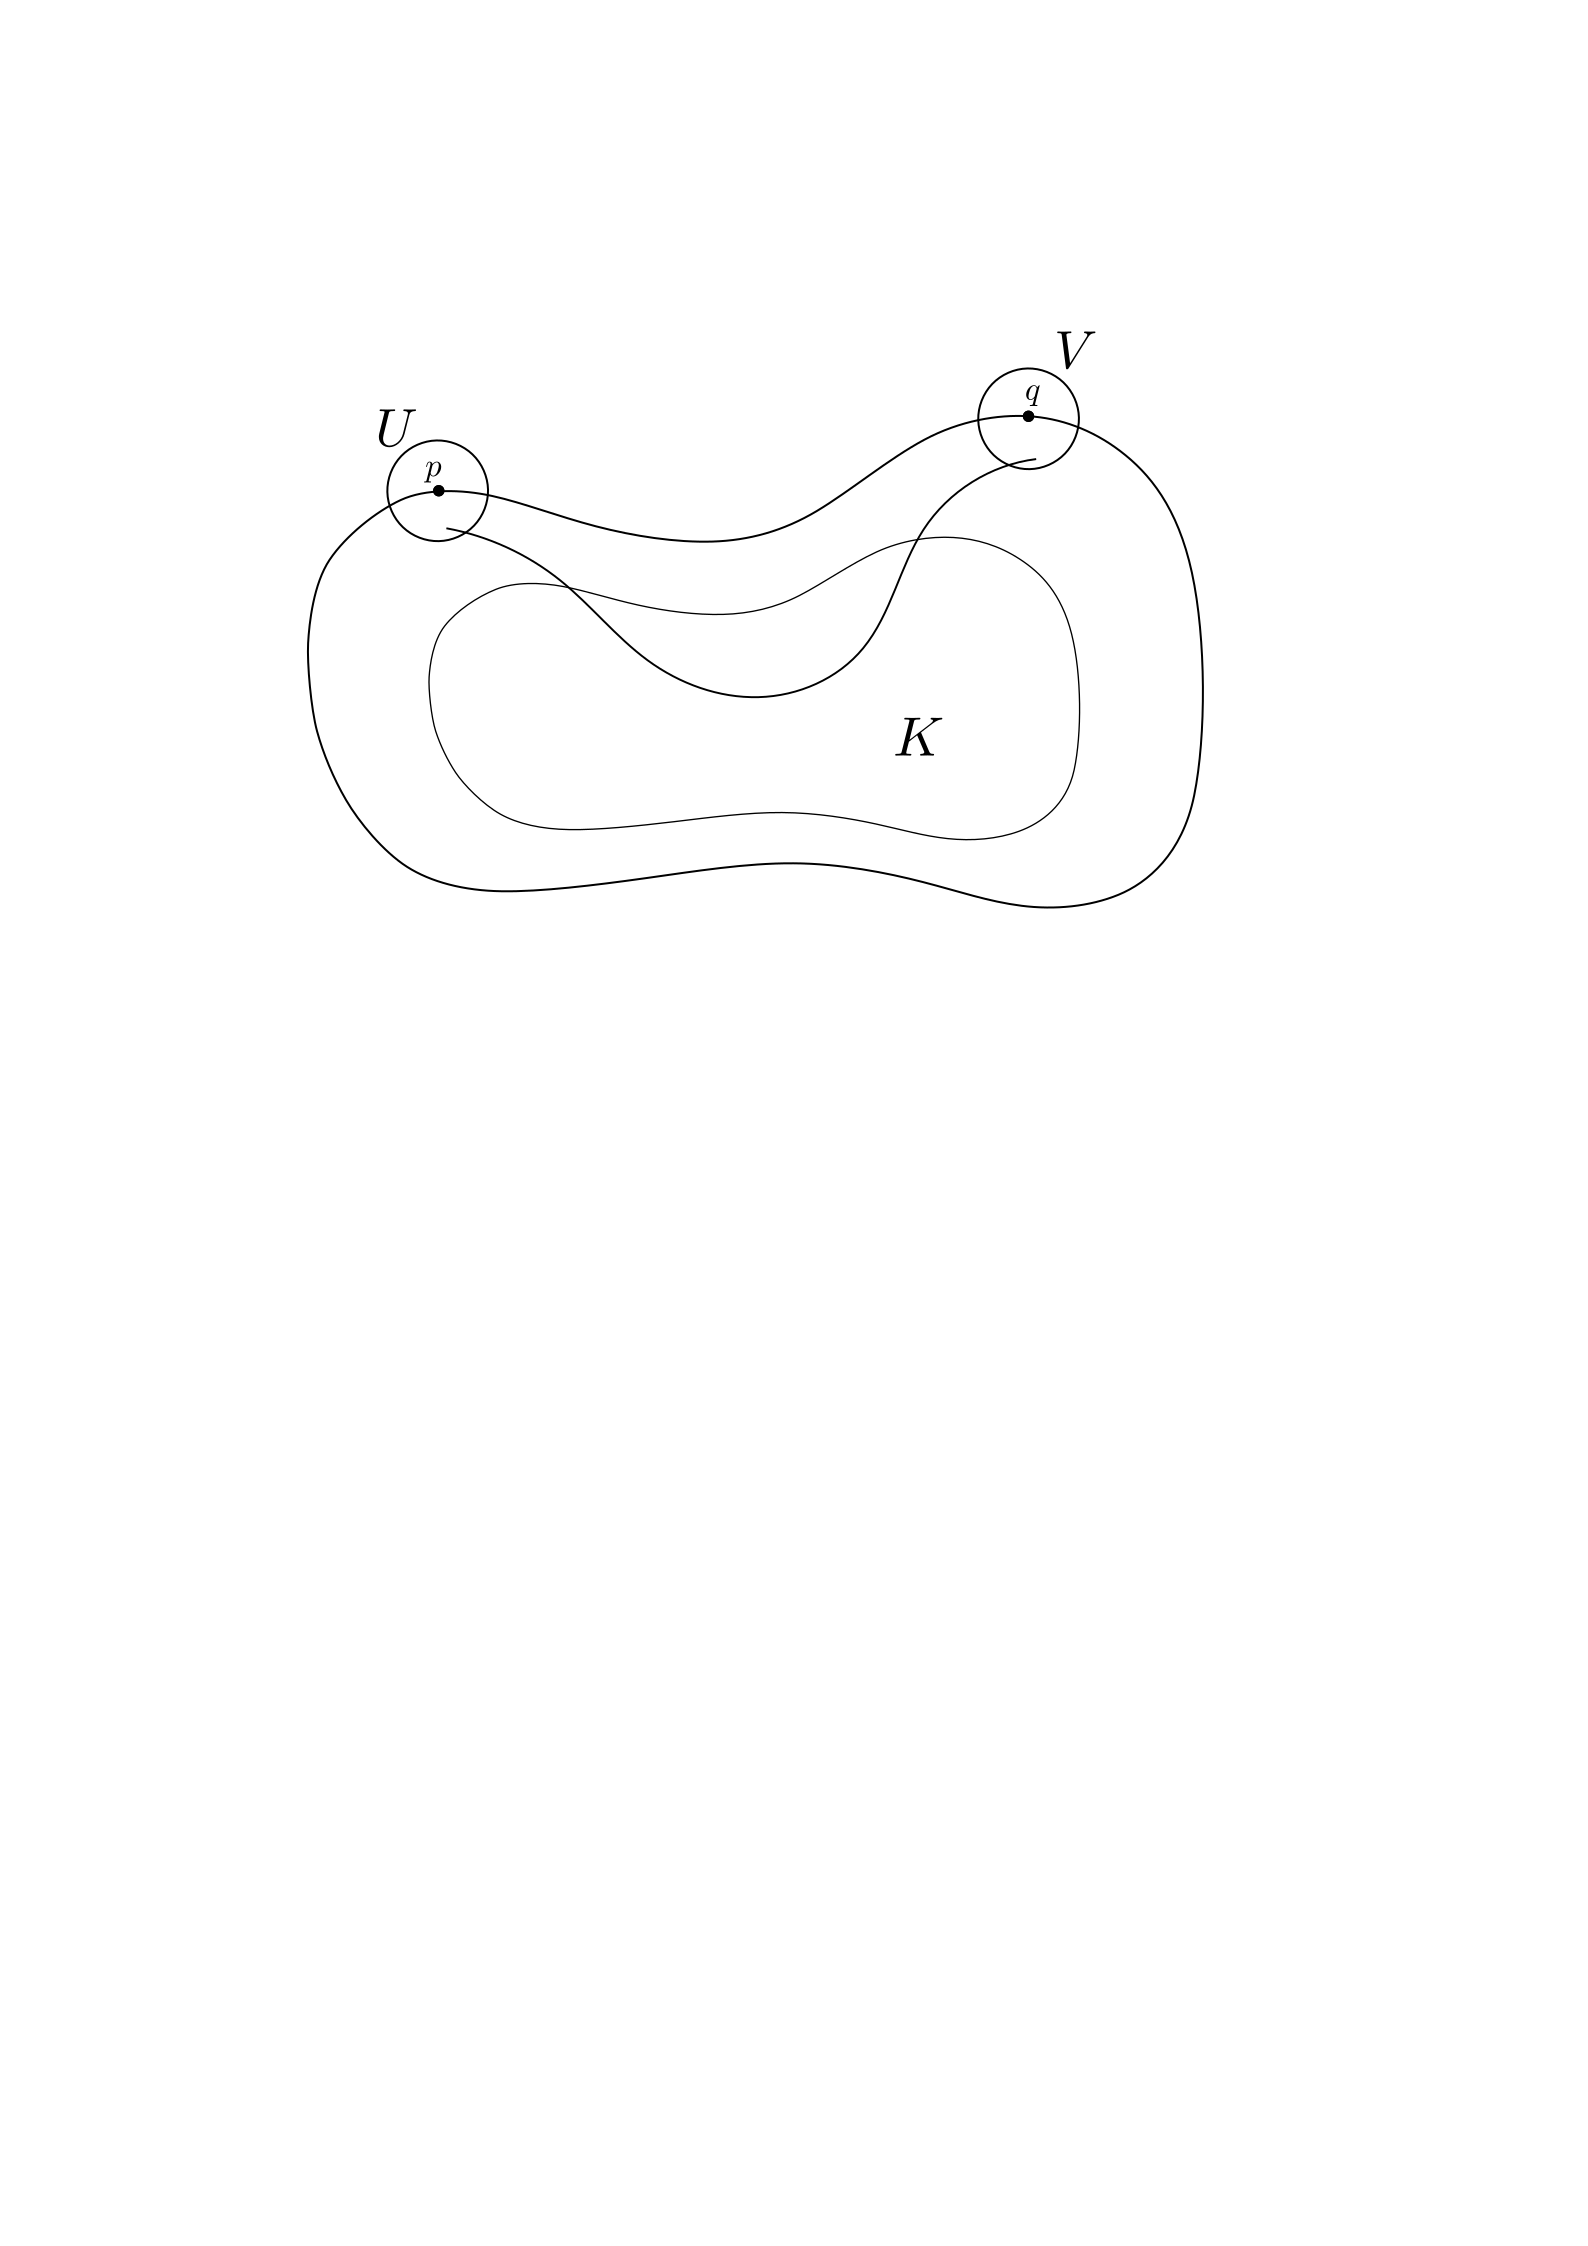
\includegraphics[width=1.05\textwidth, trim=0 18cm 0 3cm]{vis1.png}
  }
  \only<12>{
    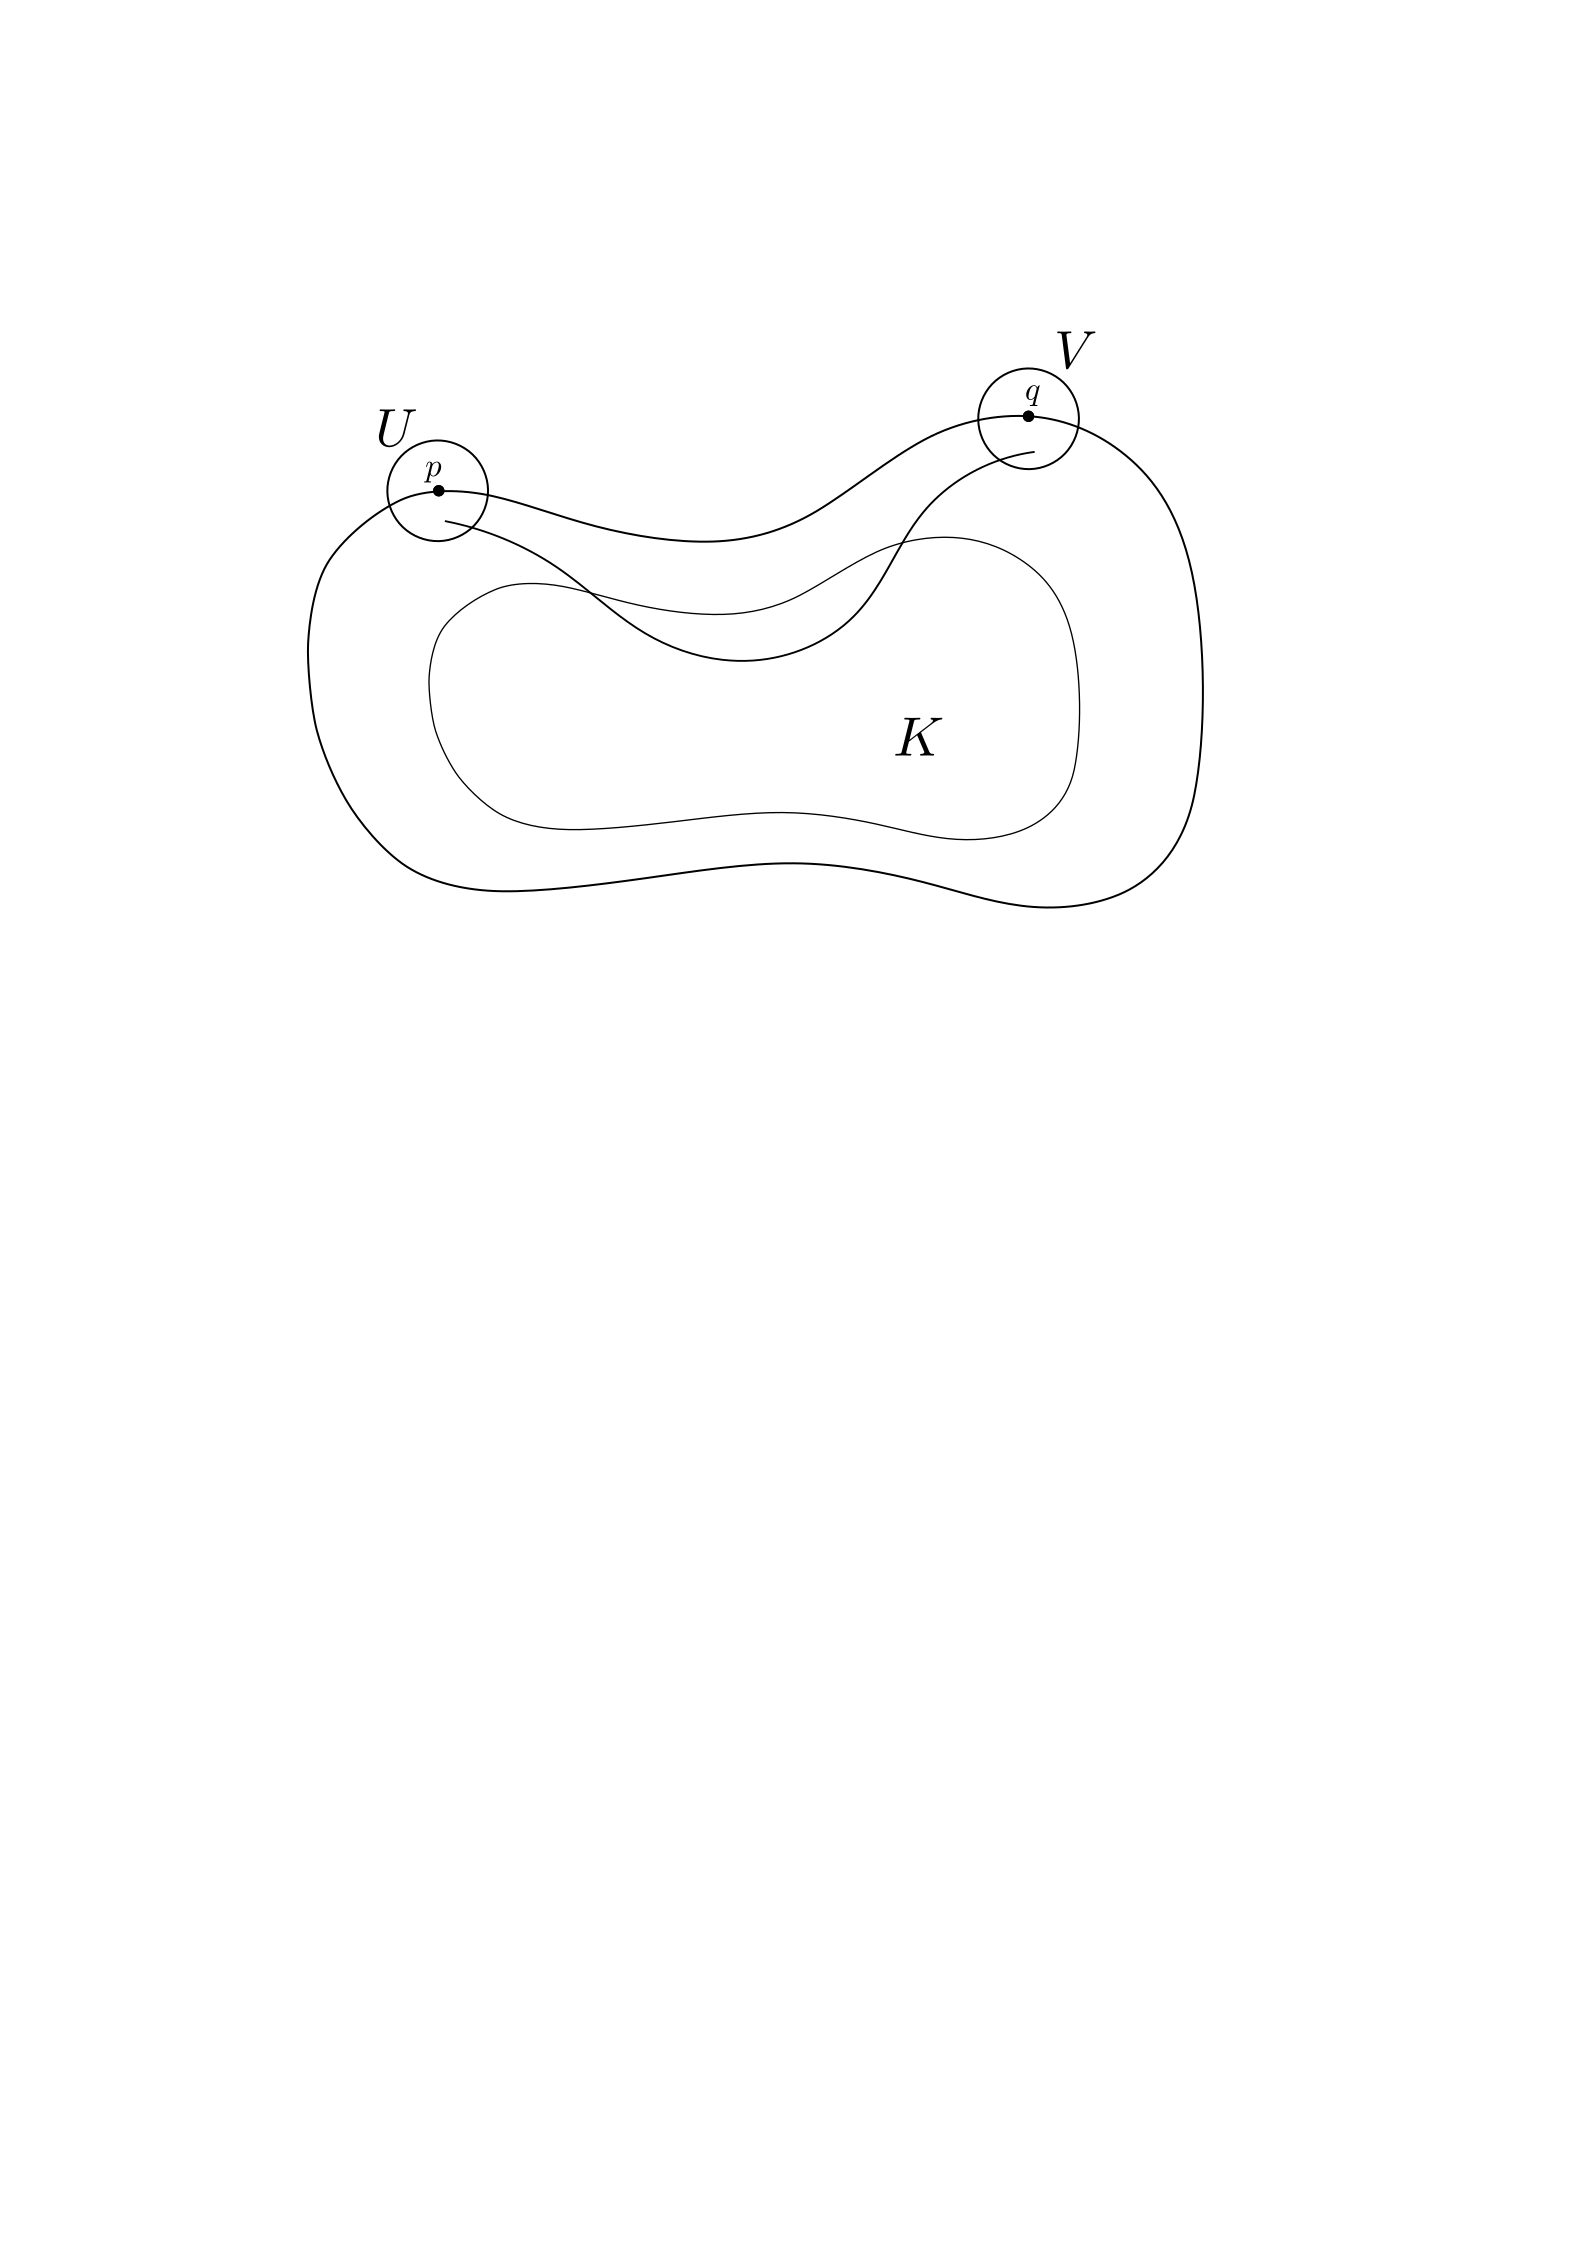
\includegraphics[width=1.05\textwidth, trim=0 18cm 0 3cm]{vis2.png}
  }
  \only<13>{
    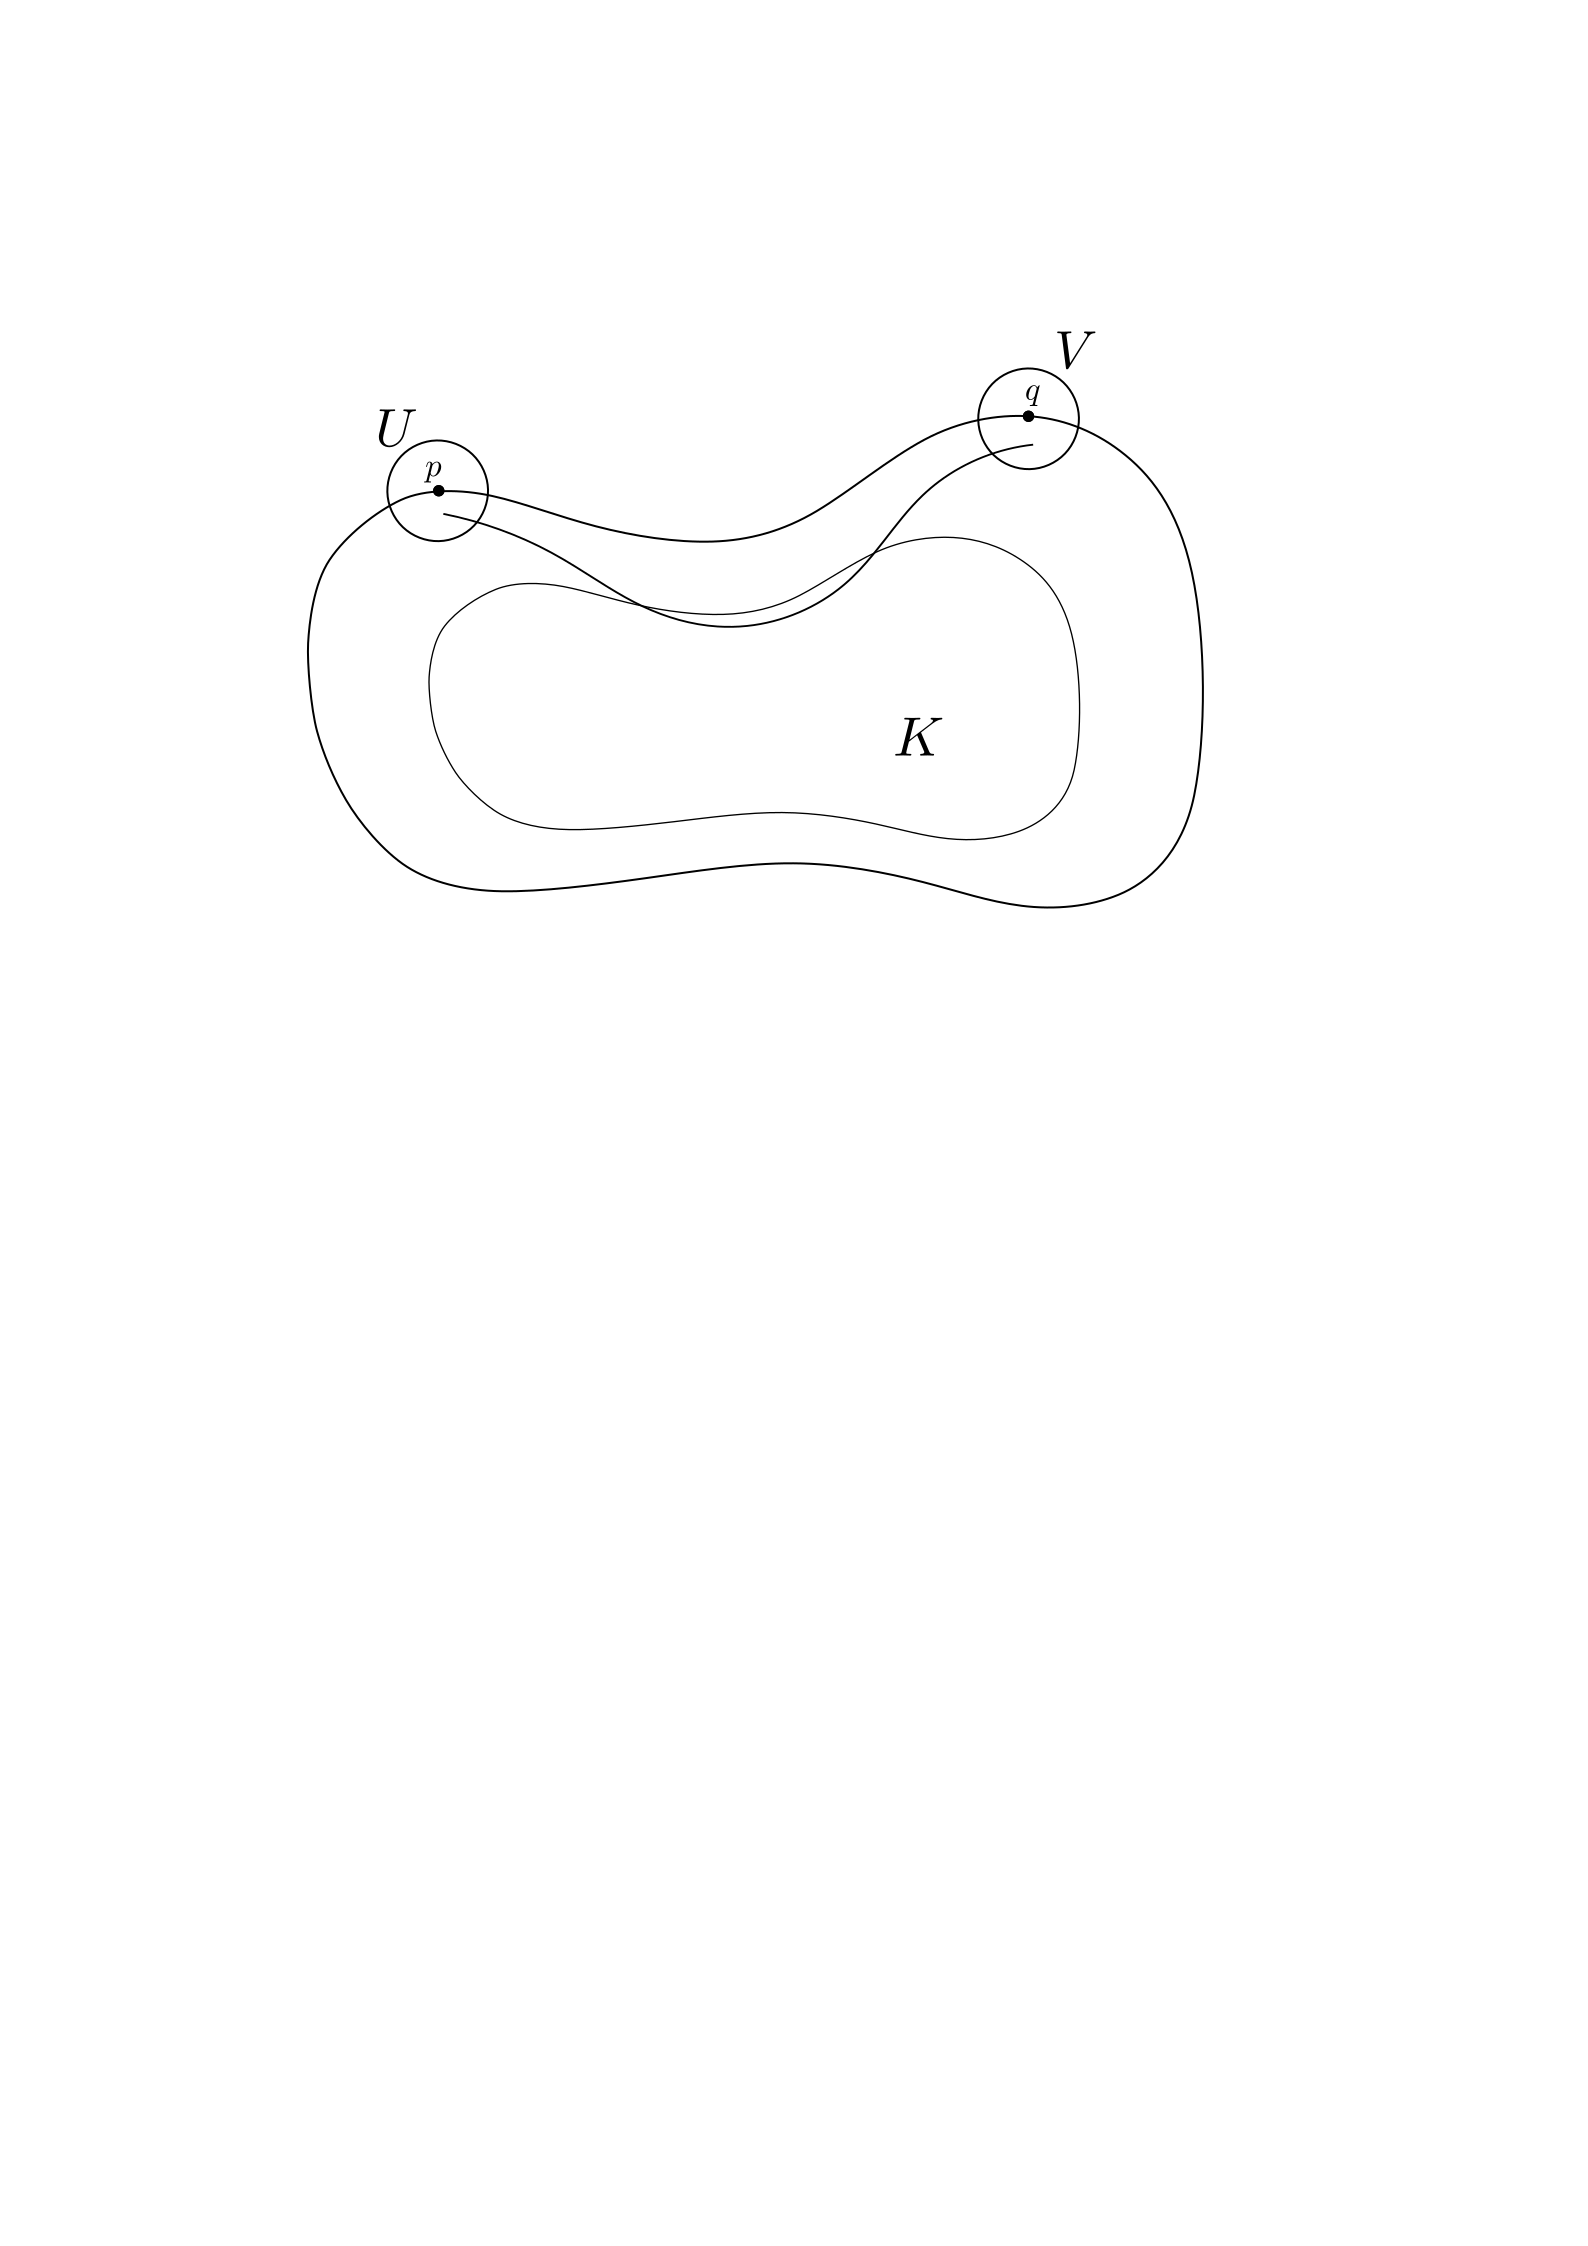
\includegraphics[width=1.05\textwidth, trim=0 18cm 0 3cm]{vis3.png}
  }
  \only<14>{
    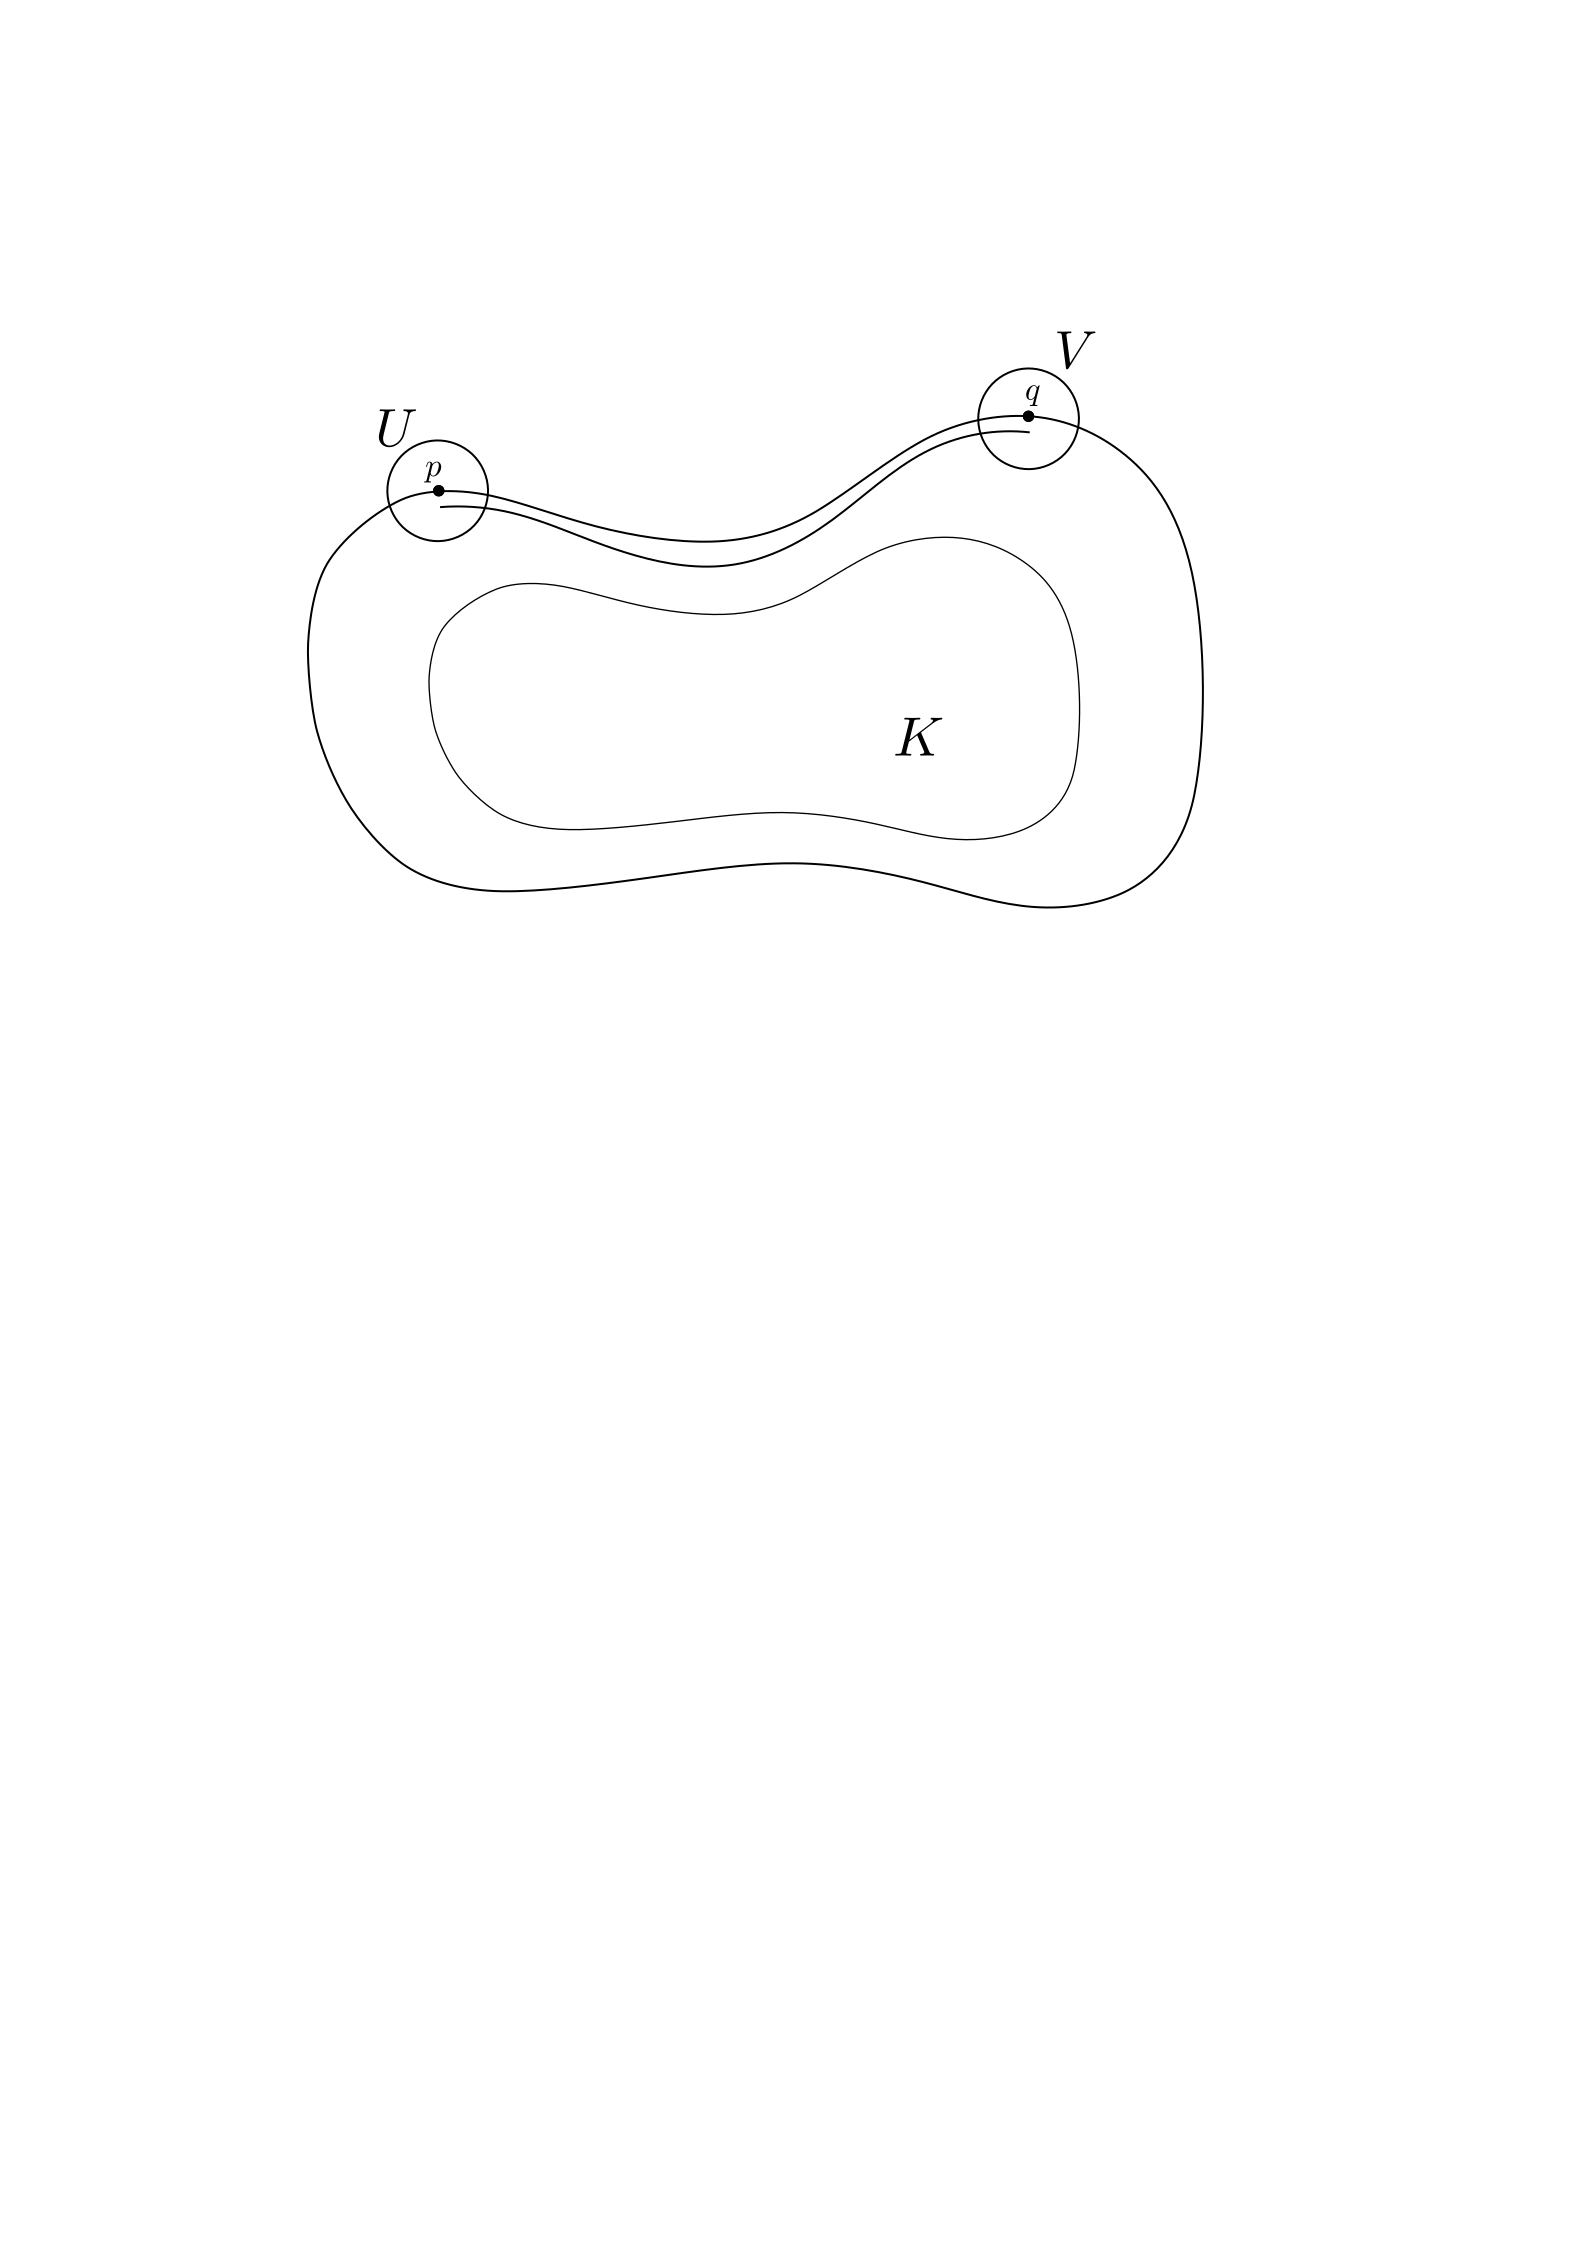
\includegraphics[width=1.05\textwidth, trim=0 18cm 0 3cm]{nonvis4.png}
  }
  \only<15>{
    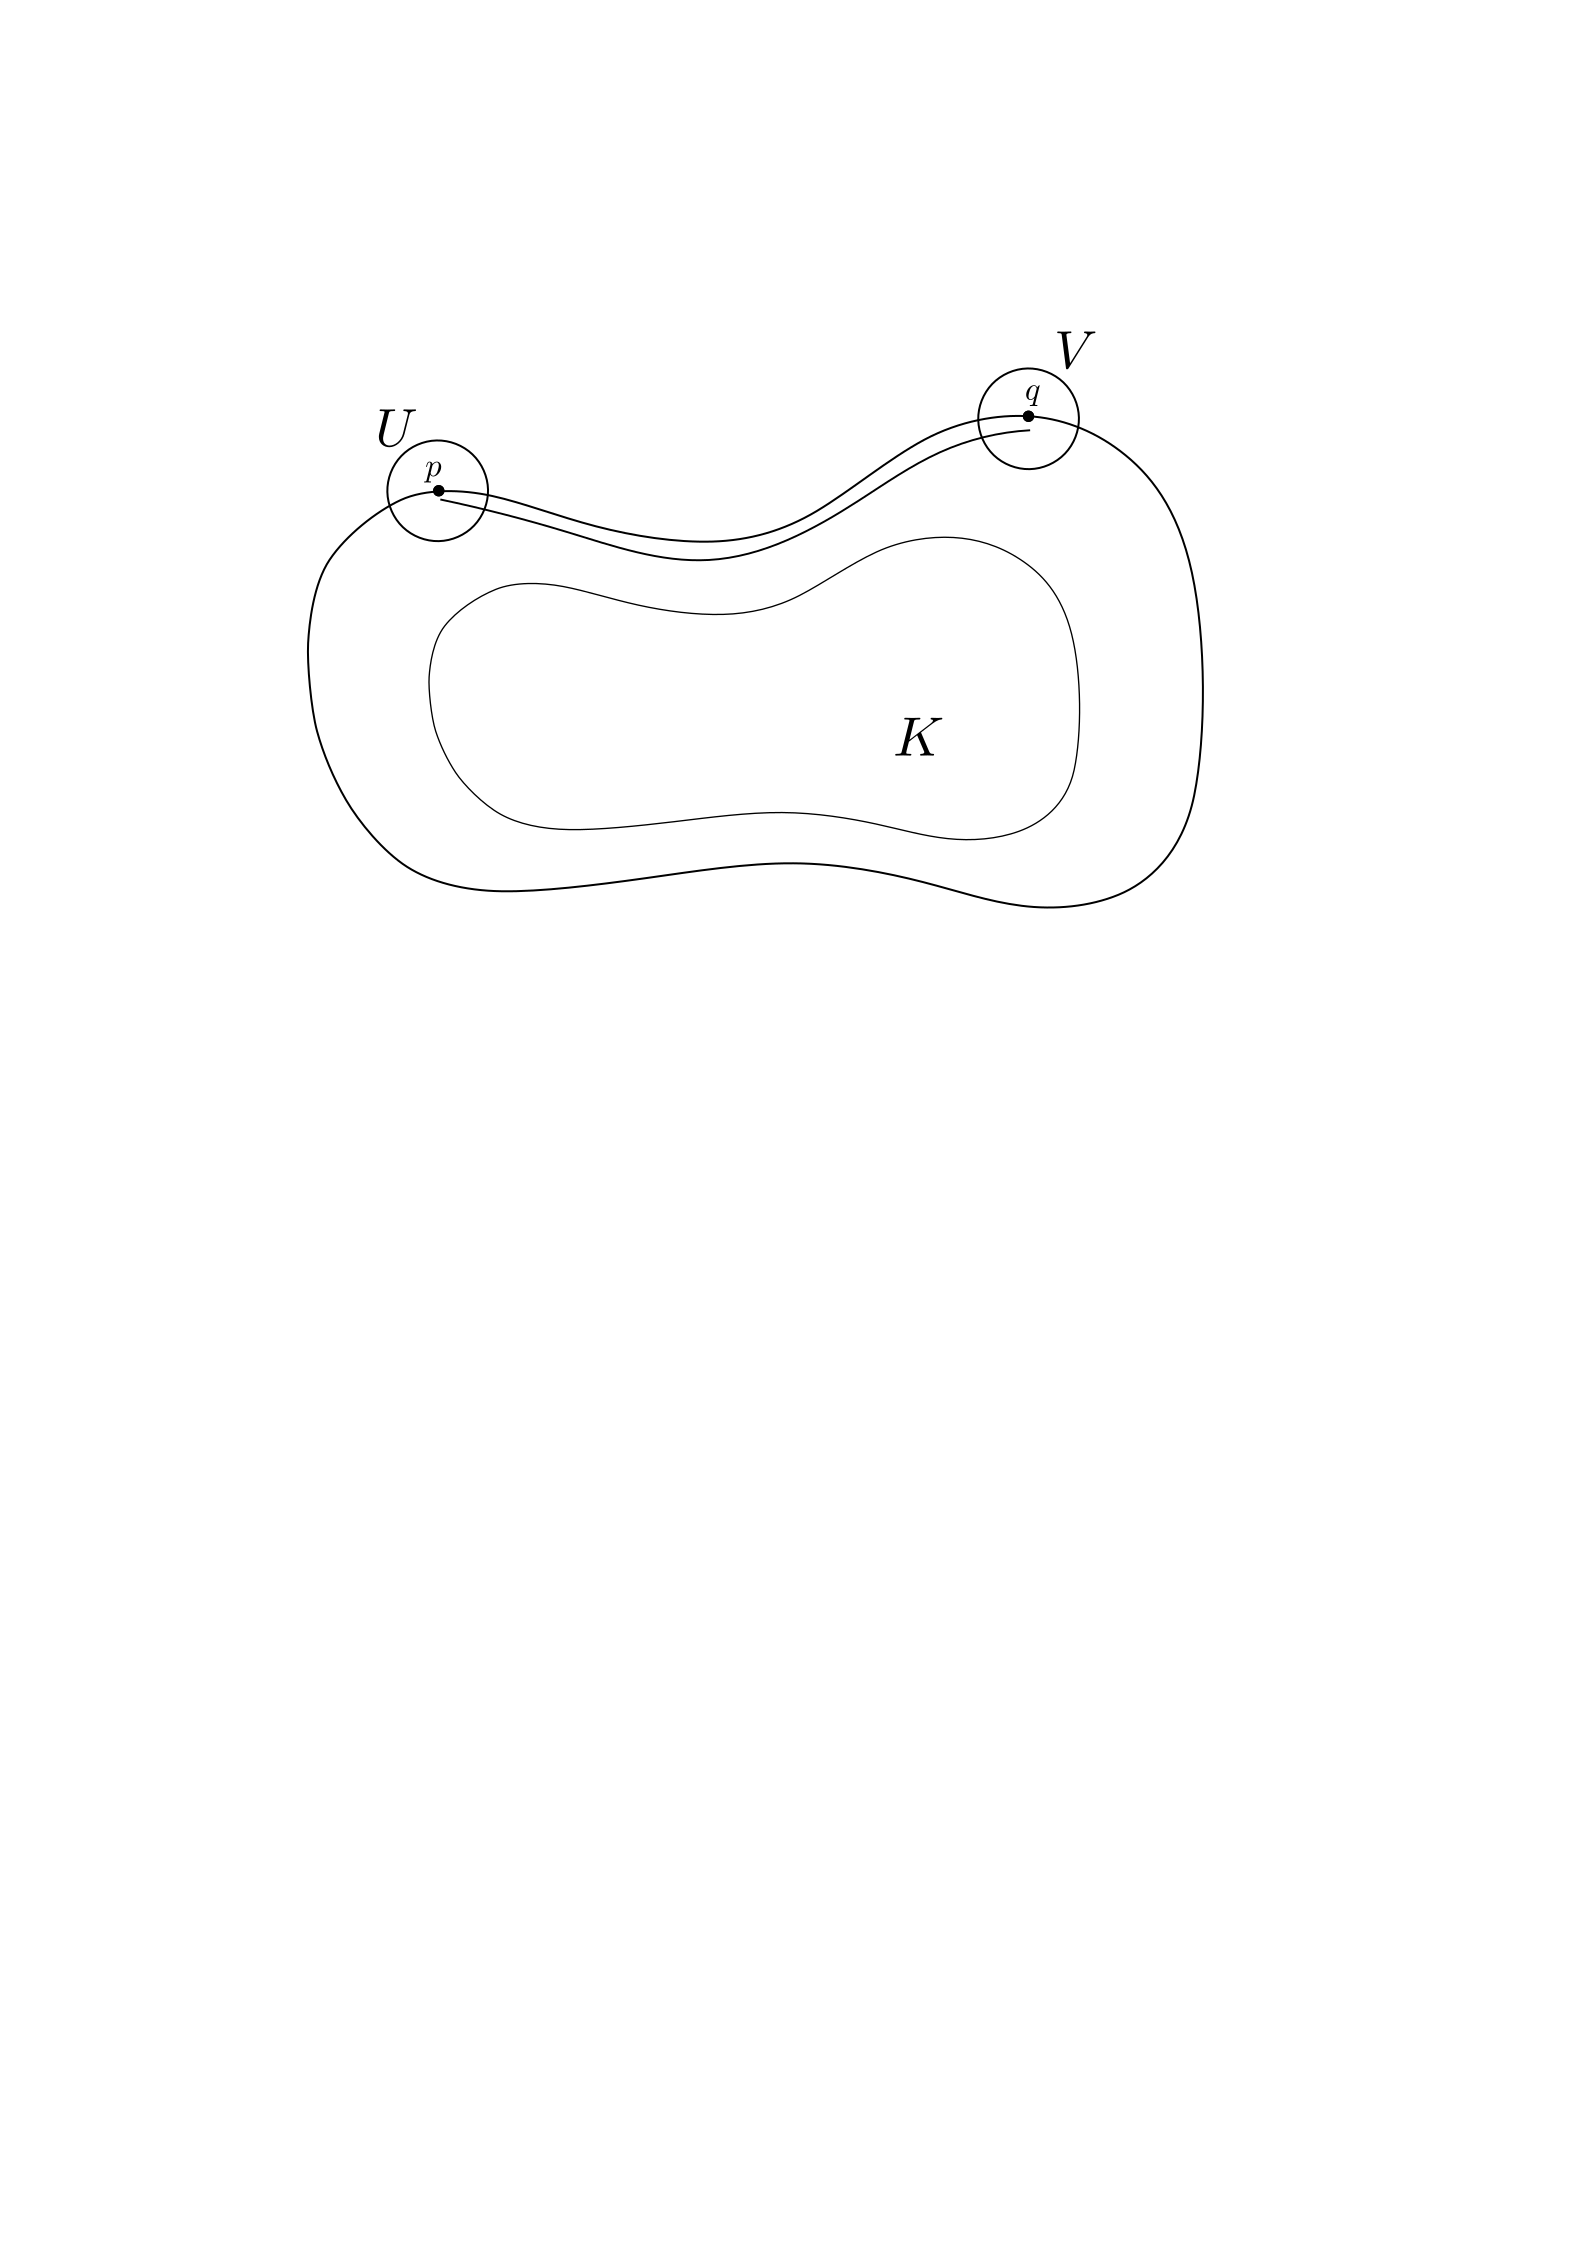
\includegraphics[width=1.05\textwidth, trim=0 18cm 0 3cm]{nonvis5.png}
  }
  \only<16>{
    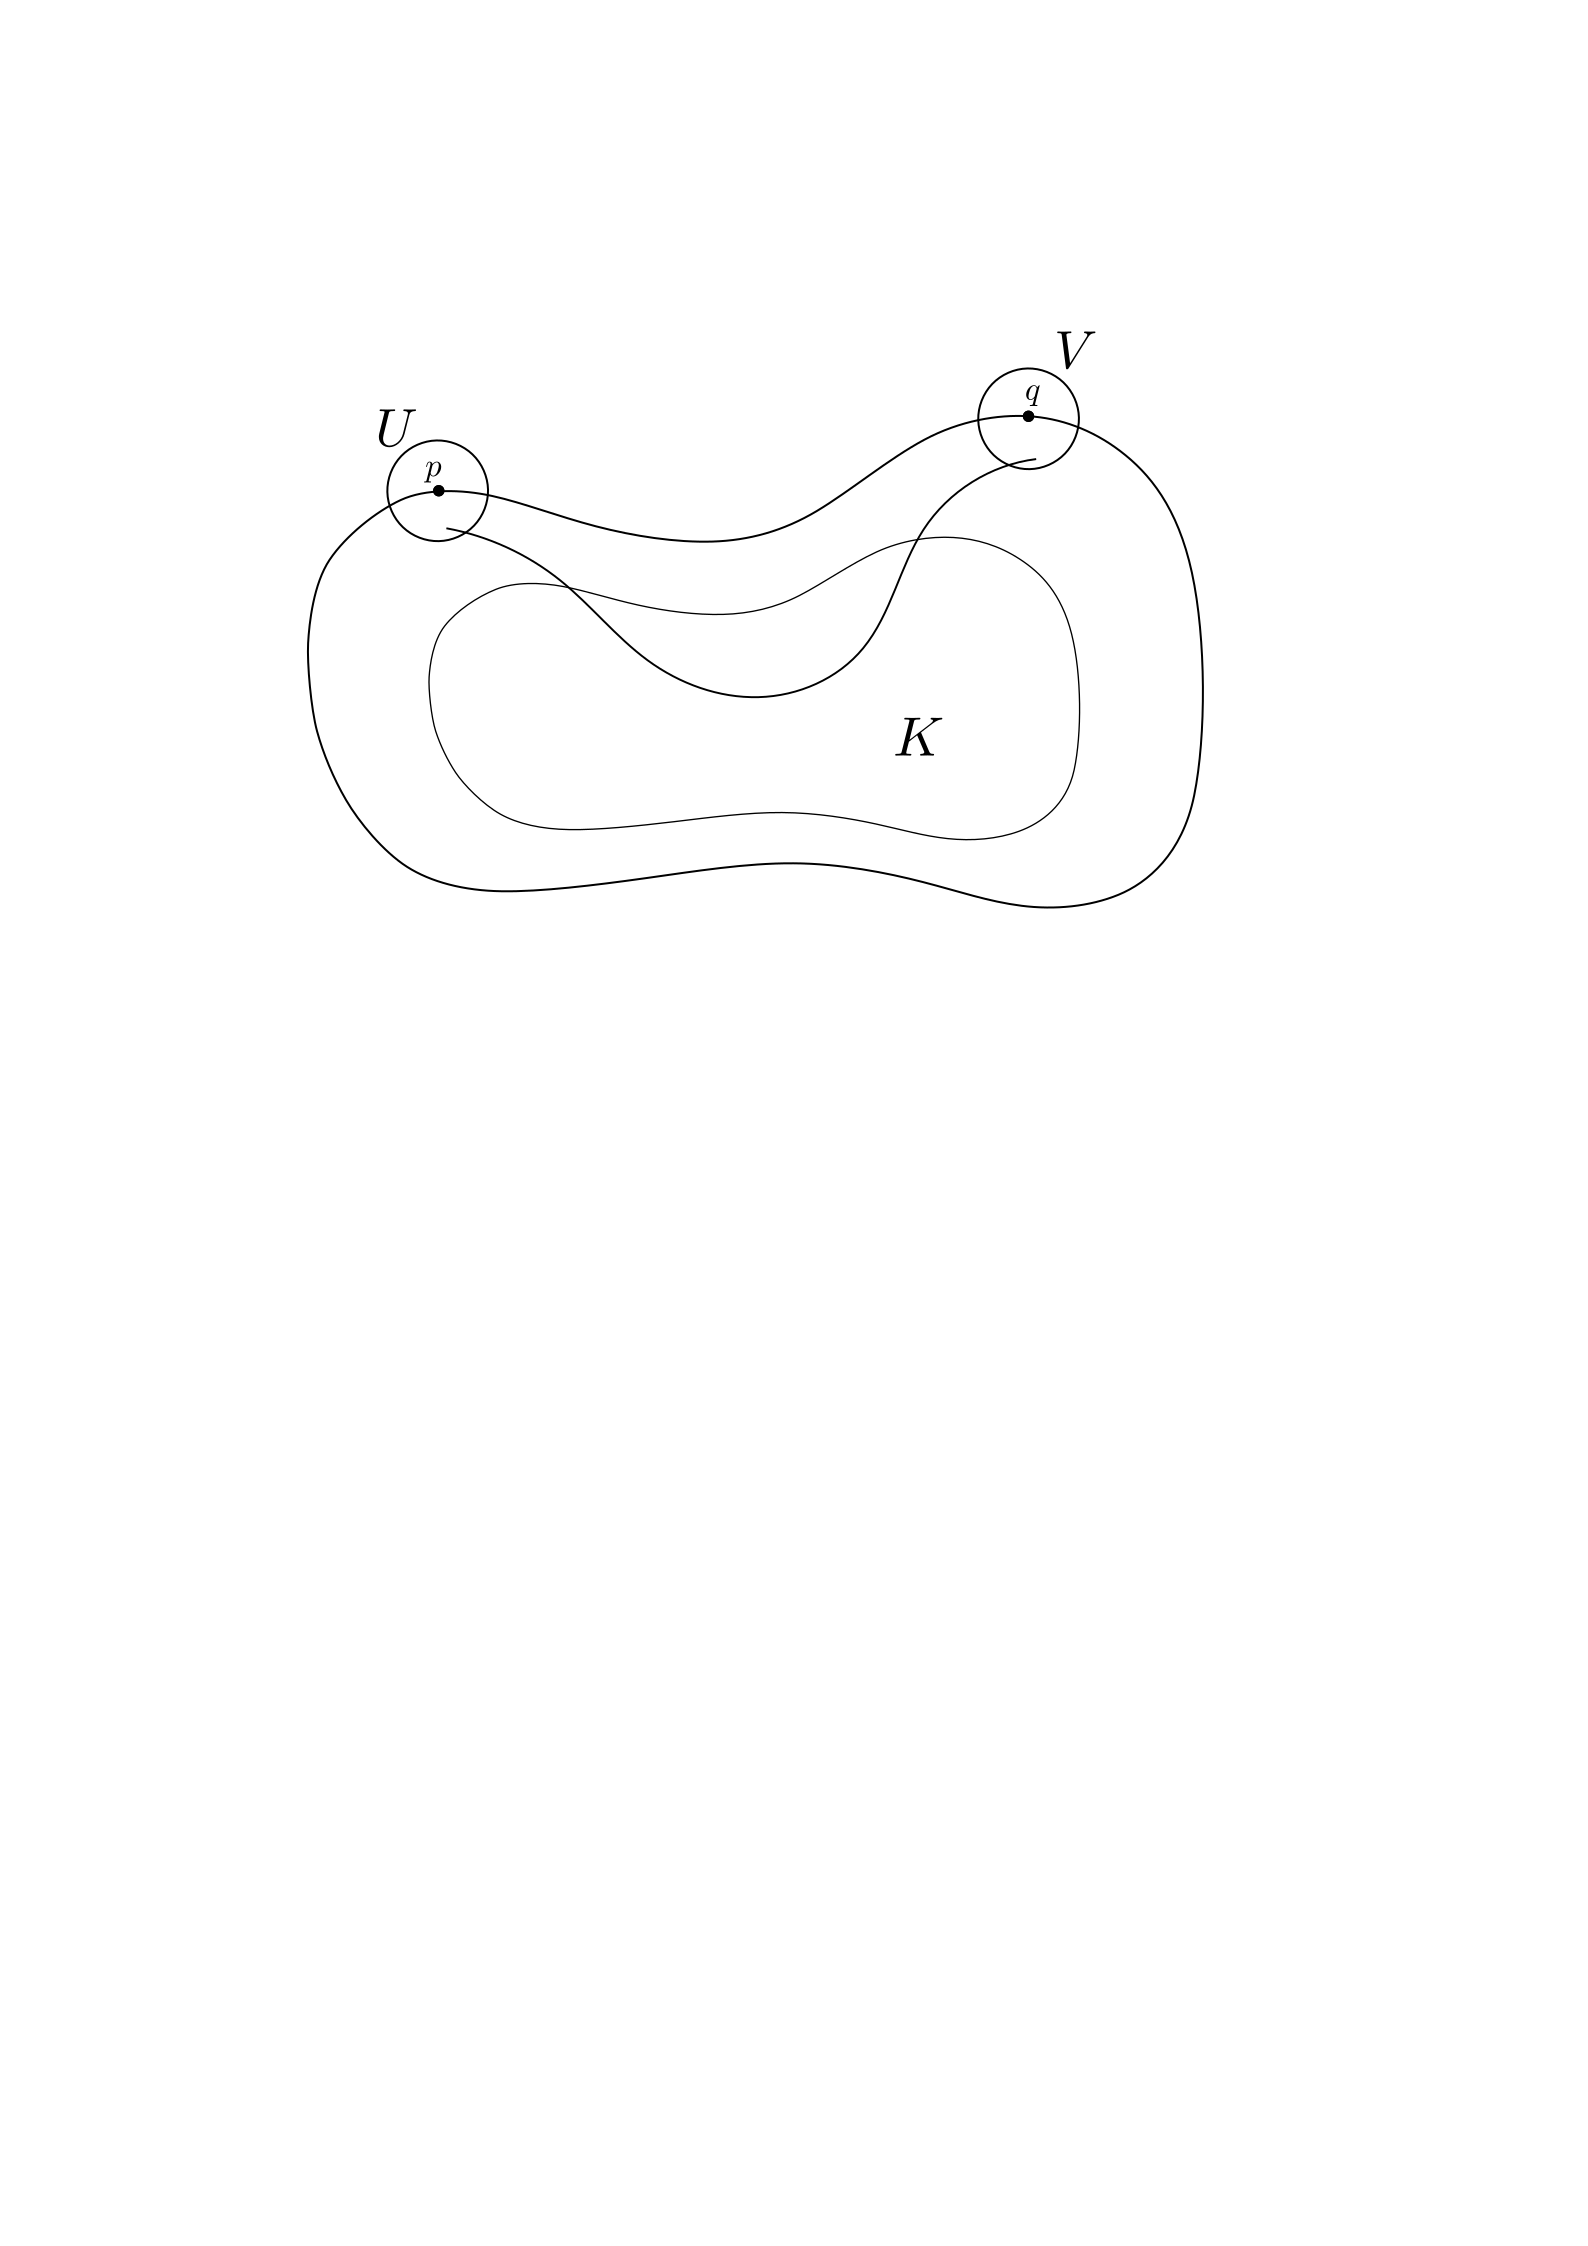
\includegraphics[width=1.05\textwidth, trim=0 16cm 0 3cm]{vis1.png}
    Condizione di visibilità: le simil-geodetiche ``curvano verso l'interno'', rimanendo dentro il compatto $K$.
  }
\end{frame}
